%%%%%%%%%%%%%%%%%%%%%%%%%%%%%%%%%%%%%%%%%%%%%%%%%%%%%%%%%%%%%%%%%%%
%                                                                 %
%   HBOOK User Guide -- LaTeX Source                              %
%                                                                 %
%   Chapter 8                                                     %
%                                                                 %
%   The following external EPS files are referenced:              %
%           pawstor.eps, hbzebra.eps                              %
%                                                                 %
%   Editor: Michel Goossens / CN-AS                               %
%   Last Mod.: 17 Feb 1995 21:45 mg                               %
%                                                                 %
%%%%%%%%%%%%%%%%%%%%%%%%%%%%%%%%%%%%%%%%%%%%%%%%%%%%%%%%%%%%%%%%%%%
 
\Filename{H1Memory-Management-and-IO-Routines}
\chapter{Memory Management and input/output Routines}
\label{HMEMORYM}
 
\Filename{H2Memory-usage-and-ZEBRA}
\section{Memory usage and ZEBRA}
\label{HMEMOUSE}

The \HBOOK{} system uses the \ZEBRA{} data manager
to store its data elements in a COMMON block \Lit{/PAWC/} 
(shared with the \KUIP{} and \HIGZ{} packages, when the latter are
also used, as is the case in \PAW{}). In fact the first task of a
\index{data structure}
\HBOOK{} user is to declare the length of this common to
\ZEBRA{} by a call to \Rind{HLIMIT}, as is seen in
figures \ref{FEX1IN} and \ref{FEX2IN}
      
In the \Lit{/PAWC/} data store, the \HBOOK,
\HIGZ{} and \KUIP{} packages have all their own
{\bf division} (see \cite{bib-ZEBRA} for
more details on the notion of divisions) as follows (see figure \ref{FPAWSTOR}):
 
\begin{DLtt}{12345}
\item[LINKS] Some locations at the beginning of
      \Lit{/PAWC/}
      \index{common {\tt/PAWC/}}\index{PAWC@{\tt/PAWC/} common}
      for \ZEBRA{} pointers.
\item[WORKS]  Working space (or division \Lit{1}) used by the
      various packages storing information in \Lit{/PAWC/}
\item[HBOOK] Division \Lit{2} of the store. Reserved to \HBOOK.
\item[HIGZ] A division reserved for the \HIGZ{} graphics package.
      This division only exists when \HIGZ{} is called.
\item[KUIP] A division reserved for the \KUIP{} user interface package.
      This division only exists when \KUIP{} is called.
\item[SYSTEM] The \ZEBRA{} system division.
      It contains some tables, as well as
      the Input/Output buffers for \Rind{HRIN} and \Rind{HROUT}.
\end{DLtt}

\begin{Fighere}
\begin{verbatim}
      COMMON/PAWC/NWPAW,IXPAWC,IHDIV,IXHIGZ,IXKU,FENC(5),LMAIN,HCV(9989)
      DIMENSION IQ(2),Q(2),LQ(8000)
      EQUIVALENCE (LQ(1),LMAIN),(IQ(1),LQ(9)),(Q(1),IQ(1))
\end{verbatim}
\begin{center}
\mbox{\epsfig{file=pawstor.eps,width=\the\textwidth}}
\end{center}
\caption{The layout of the \protect\Lit{/PAWC/} dynamic store}
\label{FPAWSTOR}
\end{Fighere}

\subsection{The use of ZEBRA}
     
Inside the \HBOOK{} division the various data elements are
stored as a \ZEBRA{} data structure, one for each ``identifier''.
In fact all identifiers (histogram or Ntuple numbers)
are stored in an ordered array in a \ZEBRA{}
bank and access to the information associated with the \HBOOK{} data
is via the {\bf reference link} at the same offset as the
identifier in the data part of the bank. The data structure for
a given element depends on its characteristics.
In any case the top bank for a given element contains the
title and other constants, while the data themselves are
stored in another bank hanging from the previous one. Sometimes
other banks are created, e.g. for automatic binning,
for storing the limits of the elements of a Ntuple and,
when a Ntuple is kept in memory, for containing the overflow
\index{projection}
of the data, for {\bf projections}, {\bf slices} and
\index{band}
{\bf bands} in the 2-dim case of for containing the {\bf errors}
\index{error}
associated to a bin. This means that each \HBOOK{} identifier
has a whole set of {\bf attributes} associated with its
\index{attribute}
existence, and when a histogram or Ntuple is written to backup
store and later reread, the {\bf complete data structure}, containing
all characteristics and attributes are retrieved.
Figure \ref{FZEBRA} shows
the \ZEBRA{} data structure for a two-dimensional histogram.
The precise layout of this bank should be of no concern to the
user. It is only shown here as an example of the underlying \ZEBRA{} structure
of \HBOOK. Note the use of the {\bf data} part of the bank for
storing attributes (e.g. title, number of bins, number of entries) as
well as of the {\bf link} part for storing the addresses to access the
associated data points (scatter plot contents, X and Y projections,
slices and bands and their associated errors).

\begin{figure}[p]
\caption[The ZEBRA data structure used for two-dimensional histograms]%
        {The \ZEBRA{} data structure used for two-dimensional histograms}
\label{FZEBRA}
\begin{center}
\mbox{\epsfig{file=hbzebra.eps,width=\the\textwidth}}
\end{center}
\end{figure}

\Filename{H2Memory-size-control}
\section{Memory size control}
\label{HMEMORYS}
 
\Shubr{HLIMIT}{(NWPAW)}
 
\Action
Defines the maximum total size \Lit{NWPAW}  of common
\Lit{/PAWC/}.
 
\Remark
\begin{UL}
\item \Rind{HLIMIT} must be called before any other \HBOOK{}
routine.
\item \HBOOK{} is compiled with a \Lit{COMMON/PAWC/} dimensioned to \Lit{10000} words.
If \Lit{NWPAW<10000}, then the default value of \Lit{10000} is assumed.
\item If \ZEBRA{} has already been initialised, \Rind{HLIMIT} must be called
with a negative argument, e.g. \Lit{CALL HLIMIT(-NWPAW)}.
\end{UL}

\Shubr{HLOCAT}{(ID,LOC*)}
 
\Action
Returns the pointer in common
\Lit{/PAWC/}
\index{common {\tt/PAWC/}}\index{PAWC@{\tt/PAWC/} common}
to the \ZEBRA{} (\cite{bib-ZEBRA}) structure,
which contains the description of a given histogram.
\begin{DLtt}{1234}
\item[{\rm\bf Input parameter:}]
\item[ID] histogram identifier
\item[{\rm\bf Output Parameter:}]
\item[LOC] Pointer to the \ZEBRA{} bank containing the histogram information.
\end{DLtt}
This routine can be useful to access directly the memory area
of a given histogram,
to extract any information that cannot be obtained with the entries
previously described.

\subsection{Space requirements}

The argument \Rarg{NWPAWC} must be given a value large enough
to accomodate in memory all histograms (1-D and 2-D) and all
Ntuple headers and buffers, i.e.

\[ \mathtt{NWPAWC} > 10000 + \sum_{i=1}^{\mathtt{NF}} S_F(i)
                           + \sum_{i=1}^{\mathtt{N1}} S_1(i)
                           + \sum_{i=1}^{\mathtt{N2}} S_2(i)
                           + \sum_{i=1}^{\mathtt{NT}} S_N(i)  \]

\begin{DLtt}{1234}
\item[NF]         Number of open files
\item[\(S_F(i)\)] 100+LREC\(_i\), where LREC is the buffer size for file \(i\),
                  as specified in a call to \Rind{HROPEN}.
\item[N1]         Number of 1-D histograms
\item[\(S_1(i)\)] Space occupied by 1-D histogram \(i\), i.e.\\
                  \Lit{40+(NCHAN+2)*PACK+IERR*(NCHAN+10)+IFUN*(NCHAN+10)}
                  \begin{DLtt}{12345}
                  \item[NCHAN] Number of channels in histogram
                  \item[PACK]  Packing factor (1. by default).
                               See parameter \Rarg{VMX} of \Rind{HBOOK1}.
                  \item[IERR]  \Lit{1} if \Rind{HBARX} called, \Lit{0} otherwise.
                  \item[IFUN]  \Lit{1} if the histogram has an associated function
                               (\Rind{HFUNC}, fits or smoothing)
                  \end{DLtt}
\item[N2]         Number of 2-D histograms
\item[\(S_2(i)\)] Space occupied by 2-D histogram \(i\), i.e.\\
                  \Lit{40+(NCHANX+2)*(NCHANY+2)*PACK} + space for projections,
                  slices and bands (which are 1-D histograms).
\item[NT]         Number of Ntuples
\item[\(S_2(i)\)] Space occupied by headers and buffers of Ntuple \(i\) 
                  (see routines \Rind{HBOOKN} and \Rind{HBNT}).
\end{DLtt}

%\subsubsection*{One-dimensional histogram}
%
%The space \Lit{NWHIST} required is \Lit{NWHIST=NWCONS1+NWCONT+NWERR+NWFUNC+6}, with:
% 
%\begin{DLtt}{123456}
%\item[NWCONS1] \Lit{16+} number of words for the title (\Lit{4} characters per
%word)
%\item[NWCONT] \Lit{(NCX+2)/NPACK  +  10}  where \Lit{NPACK} is the packing factor.\\
%If one word is allocated per channel, then \Lit{NPACK=1}.\\
%If eight bits per channel are used on a 32 bits machine, then \Lit{NPACK=4}.
%\Lit{NCX} is the number of channels.
%\item[NWERR] \Lit{NCX+10} if \Rind{HBARX} or \Rind{HPAKE} are called.
%\item[NWFUNC] \Lit{NCX+10} if there is an associated function.
%\end{DLtt}
% 
%\subsubsection*{Two-dimensional histogram}
%
%The space \Lit{NWHIST} required is defined by the following parameters:
% 
%\begin{DLtt}{123456}
%\item[NWCONS2] \Lit{NWCONS1 + 4}.
%\item[NWCONT] \Lit{(NCX+2)*(NCY+2)/NPACK + 10}
%where \Lit{NCX} and \Lit{NCY} are the number of
%channels in \Lit{X} and \Lit{Y} respectively.
%\item If projections, bands or slices are defined, one should add for
%each projection, etc the corresponding number of words
%(\Lit{NWCONT+NWERR+6}).
%\end{DLtt}
 
\Filename{H2Directories}
\section{Directories}
\label{HDIRECTO}
 
\HBOOK{} histogram data are kept in a \ZEBRA{}
tree structure similar to the directory structure
of the Unix file system.
\index{Unix}%
\index{ZEBRA}%
\index{directory}
Note that the \ZEBRA{} RZ package uses the same conventions. (In fact,
\HBOOK{} uses the \ZEBRA{} RZ package to manage files).
With this convention, all references to histograms
are still made using an integer identifier, but this identifier
is relative to a {\bf directory}.
\HBOOK{} initially sets the current directory to be \Lit{//PAWC}.
\index{common {\tt/PAWC/}}\index{PAWC@{\tt/PAWC/} common}
This directory remains the current directory until changed either explicitly
or implicitly by one of the calls described below.
As with the Unix file system the current directory can be
a subdirectory, e.g. \Lit{//PAWC/L1},
\Lit{//PAWC/L1/L21} and \Lit{//PAWC/L1/L22}.
 
These \HBOOK{} directories can reside in the local memory
of the computer (i.e. the \Lit{PAWC} common,
\index{common {\tt/PAWC/}}\index{PAWC@{\tt/PAWC/} common}
or they can be stored on a local (\Lit{//LUN1}) or
remote disk file system (\Lit{//VXCRNA}).
They can even be dynamically created by a ``producer'' in
the memory of a remote computer and ''shared'' by
that machine with the user's machine via global section (VMS)
or shared memory (Unix).

\begin{Fighere}
\begin{XMP}
                                                          HMDIR HCDIR HLDIR HDDIR HPDIR
--------    //PAWC                     local memory         X     X     X     X     X
|      |    //LUN1                     local disk           X     X     X     X     X
| USER |    //VXCRNA ---- telnet (rsh) remote disk          X     X     X
|      |    //GLOSEC ---- tcp/ip ---   global section(VMS)  X     X     X
--------    //SHARE  ---- tcp/ip ---   shared memory(Unix)  X     X     X
\end{XMP}
\caption[Different kinds of HBOOK directories]%
        {Different kinds of \HBOOK{} directories}
\label{FDIRKIND}
\end{Fighere}

\finalnewpage
\Shubr{HMDIR}{(CHPATH,CHOPT)}
 
\Action
Make a new subdirectory below the current directory. 
This command works with all five different kinds of directories 
described in figure \ref{FDIRKIND}.
 
\begin{DLtt}{123456}
\item[{\rm\bf Input parameters:}]
\item[CHPATH] Character
variable or constant containing the name of the subdirectory.
\item[CHOPT] Character variable specifying the option chosen.
If \Lit{CHOPT='S'} then the current directory is changed to the new
directory.
\end{DLtt}
 
%\finalnewpage%%%%%%%%%%%%%%%%%%%%%%%%%%%%%%%%%%%%%%%%%%%%%%%%%%%%%%%%%%%%%

\Shubr{HCDIR}{(*CHPATH*,CHOPT)}
 
\Action
Change the current directory.
This command works with all five different kinds of directories 
described in figure \ref{FDIRKIND}.
 
\begin{DLtt}{123456}
\item[{\rm\bf Input parameters:}]
\item[CHPATH] Character
variable or constant containing the name of the directory which
is to become the current directory (default action if \Lit{CHOPT=' '}).
\item[CHOPT] Character variable specifying the option chosen.\\
\Lit{' '} Set new directory.\\
\Lit{'R'} Read the name of the current directory.
\item[{\rm\bf Output Parameter}]
\item[CHPATH] Character
variable containing the name of the current directory (\Lit{CHOPT='R'}).
\end{DLtt}
 
\begin{XMPt}{Setting RZ directories}
CALL HCDIR('//PAW/CDET',' ')     ! {\rm Go to directory with given absolute pathname}
                                   
CALL HCDIR('TPC',' ')            ! {\rm Go to directory with given relative pathname}
                                 ! {\rm we are now in} //PAW/CDET/TPC

CALL HCDIR('//PAW/CDET/TPC',' ') ! {\rm Equivalent to 1+2 above}

CALL HCDIR('\bs',' ')              ! {\rm Go to parent directory, i.e.} //PAW/CDET

CALL HCDIR('TPC',' ')            ! {\rm Go to TPC subdirectory again}

CALL HCDIR ('\bs{}VERTEX',' ')       ! {\rm Go to directory} //PAW/CDET/VERTEX
                                 ! {\rm i.e. one level up then one down again}
\end{XMPt}

This concept of directories also applies to
the direct access files when using \Rind{HRFILE}, \Rind{HRIN}
and \Rind{HROUT}.

\finalnewpage
\Shubr{HLDIR}{(CHPATH,CHOPT)}
 
\Action
List the contents (identifiers, type of histograms
and titles) of a \HBOOK{} directory.
This command works with all five different kinds of directories 
described in figure \ref{FDIRKIND}.
 
\begin{DLtt}{123456}
\item[{\rm\bf Input parameters:}]
\item[CHPATH] Character
variable or constant containing the name of the directory to be listed.
\Lit{CHPATH=' '} stands for the current directory.
\item[CHOPT] Character variable specifying the chosen option.
\begin{DLtt}{1234}
\item[' '] List only the top directory.
\item['A'] List all Ntuple extentions.
\item['I'] \Rind{HINDEX} option selected instead of simple list.
\item['N'] List only the Ntuples.
\item['R'] List using RZ format.
\item['S'] Sort the directory entries.
\item['T'] List the complete subdirectory tree starting
from the specified directory.
\end{DLtt}
\end{DLtt}
\newpage 
\begin{XMPt}{List all existing directories in //PAWC} 
CALL HLDIR ('//PAWC','T')
\end{XMPt}

\Shubr{HDDIR}{(CHPATH))}
 
\Action
Delete a (sub)directory from memory or local disk.
 
\begin{DLtt}{123456}
\item[{\rm\bf Input parameter:}]
\item[CHPATH] Character variable or constant specifying 
              the pathname of the (sub)directory to delete.\\
              \Lit{CHPATH=' '} stands for the current directory.
\end{DLtt}
 
%\finalnewpage%%%%%%%%%%%%%%%%%%%%%%%%%%%%%%%%%%%%%%%%%%%%%%%%%%%%%%%%%%%%%

\Shubr{HPDIR}{(CHPATH,CHOPT)}
 
\Action
Print the contents of a directory (This routine calls
\Rind{HPRINT}).
This routine works only for directories in local memory
or remote RZ files accessed opened via \Rind{XZRZOP} (see
the CSPACK manual~\cite{bib-CSPACK} for more information).
 
\begin{DLtt}{123456}
\item[{\rm\bf Input parameters:}]
\item[CHPATH] Character variable or constant specifying 
              the pathname of the directory to be printed.\\
              \Lit{CHPATH=' '} stands for the current directory.
\item[CHOPT] Character variable specifying the option chosen.
\begin{DLtt}{1234}
\item[' '] Print the contents of the top directory.
\item['I'] Print an index.
\item['T'] Print the complete directory tree (i.e. the top
directory and its subdirectories).
\end{DLtt}
\end{DLtt}
 
\begin{XMPt}{Printing list of histograms} 
CALL HPDIR ('//PAWC','T') ! Print list of all histograms in //PAWC

CALL HPDIR (' ',' ')      ! Print list of all histograms in current directory

CALL HPRINT(0)            ! Print histograms in current directory
\end{XMPt}


\Shubr{HLNEXT}{(*IDH*,CHTYPE*,CHTITL*,CHOPT)}
 
\Action
Scan the contents of the current directory in memory or on an 
RZ file.
 
\begin{DLtt}{123456}
\item[{\rm\bf Input parameters}]
\item[IDH] Must be zero for first call
\item[CHTYPE] Character variable specifying items to be scanned.
  \begin{DLtt}{123}
    \item['1'] include 1-D histograms
    \item['2'] include 2-D histograms
    \item['N'] include Ntuples
    \item['D'] include subdirectories
    \item[' '] include everything, i.e., equivalent to \Lit{'12ND'}.
  \end{DLtt}
\end{DLtt}
\newpage\begin{DLtt}{123456}
\item[{\rm\bf Output parameters}]
\item[IDH] On return contains identifier of next histogram.
           When all histograms are processed, a value of zero
           is returned.
\item[CHTYPE] Character variable specifying type of histogram.
  \begin{DLtt}{123}
    \item['1']   1-dimensional
    \item['2']   2-dimensional
    \item['N']   Ntuple
    \item['D']   subdirectory
    \item['?']   unknown.
  \end{DLtt}
\item[CHTYPE] Character variable containing title
              or subdirectory name.
\end{DLtt}

\begin{XMPt}{Scan content of current directory}
      IDH=0
  1   CONTINUE
      CALL HLNEXT(IDH,CHTYPE,CHTITL,CHOPT)
      IF(IDH.NE.0) THEN
         ... process
         GOTO 1
      ENDIF
\end{XMPt}

\finalnewpage%%%%%%%%%%%%%%%%%%%%%%%%%%%%%%%%%%%%%%%%%%%%%%%%%%%%%%%%%%%%%
 
\Shubr{HRDIR}{(MAXDIR,CHDIR*,NDIR*)}
 
\Action
Returns the list of subdirectories of the current working directory.
This command works with all five different kinds of directories 
described in figure \ref{FDIRKIND}.
 
\begin{DLtt}{123456}
\item[{\rm\bf Input parameter}]
\item[MAXDIR] Length of the character array \Lit{CHPATH}.
\item[{\rm\bf Output parameters}]
\item[CHDIR*] Character array which will contain the names
of the subdirectories of the current working directory.
\item[NDIR*]
Actual number of subdirectories present in the current working directory.
If this number is greater than \Lit{MAXDIR}, only the first
\Lit{MAXDIR} subdirectory names will be returned in array \Lit{CHDIR}.
\end{DLtt}
 
The use of directories is illustrated below:
\begin{XMPt}{Example of use of directories}
      PROGRAM MAIN
*
      COMMON/PAWC/H(20000)
      CALL HLIMIT (20000)
      CALL HBOOK1 (10,'Energy distribution',100,0.,300.,0.)
           "   "
*
      CALL USECAL
           "   "
      CALL HFILL (10,EDER,0.,1.)
           "   "
      CALL HISTDO
           "   "
      END
      SUBROUTINE USECAL
*
*        Make a new directory ECAL and set the new current directory
*
          CALL HMDIR ('ECAL','S')
*
*        Create a new histogram with ID=10 in the new directory
*
          CALL HBOOK1 (10,'My histogram',50,-5.,5.,0.)
           "   "
          CALL HFILL (10,UX,0,1.)
 
           "   "
*         Go back to the parent directory
*
          CALL HCDIR ('\bs','  ')
           "   "
      END
\end{XMPt}

\finalnewpage%%%%%%%%%%%%%%%%%%%%%%%%%%%%%%%%%%%%%%%%%%%%%%%%%%%%%%%%

\Filename{H2Input-Output-Routines}
\section{Input/Output Routines}
\label{HINOUTPU}
\index{input}
\index{output}
\index{I/O}
 
\HBOOK{} files are in fact \ZEBRA{} RZ files~\cite{bib-ZEBRA}.
\index{ZEBRA!RZ package}%
\index{RZ package of ZEBRA}%
Input/output error return codes are available
vin the \ZEBRA{} communication vector \Lit{IQUEST},
and the user should consult the RZ manual for their meaning.
\index{error!return codes|see {{\tt IQUEST}}}
\index{IQUEST@{\tt IQUEST} communication vector}
Both disk and memory resident files are supported, the latter being
particularly useful in online applications,
\index{online}
where histogram data have to be shared between different processes.
 
\index{direct access file}

\HBOOK{} files are written in Zebra exchange format and thus
need not be converted when transferred between different computer
systems using binary ftp (see section~\ref{sec:histogram-transfer}),
or accessed over the network using
a distributed file system such as \Lit{AFS} or \Lit{NFS}.
 
\subsection*{Reading and writing histograms to a direct access file}
 
\Shubr{HRPUT}{(ID,CHFILE,CHOPT)}
 
\Action
Write a histogram to a given direct  access  file.
This routine cannot be used for Ntuples.
\index{Ntuple}
 
\begin{DLtt}{123456}
\item[{\rm\bf Input parameters:}]
\item[ID] Histogram identifier.
          \Lit{ID=0} writes all histograms in the current directory to
          the output file.
\item[CHFILE] Character variable or constant defining the filename.\\
          If \Lit{CHFILE=' '} the histogram is saved in the
          current working directory on disk.
\item[CHOPT] Character option specifying the desired option.
          \begin{DLtt}{123}
             \item['N'] Write the histogram to a New file.
             \item['T'] Can be used together with \Lit{ID=0}. 
                        All histograms in the current directory and all 
                        subdirectories in memory are written to the output file.
            \item['U'] Write the histogram to an already existing \HBOOK{} file.
                       When an histogram with the same identifier already 
                       exists on the output file, then a new cycle is added.
          \end{DLtt}
\end{DLtt}
 
\Shubr{HRGET}{(ID,CHFILE,CHOPT)}
 
\Action
Read a histogram from a given direct  access  file.
This routine cannot be used for Ntuples.
\index{Ntuple}
 
\newpage\begin{DLtt}{123456}
\item[{\rm\bf Input parameters:}]
\item[ID] Histogram identifier.
          \Lit{ID=0} read all histograms into the current directory.
\item[CHFILE]
          Character variable or constant defining the input filename.\\
          If \Lit{CHFILE=' '} the histogram is read from the
          current working directory on disk.
\item[CHOPT]
          Character option specifying the desired option.
          \begin{DLtt}{1234}
              \item['A'] Add to the current histogram in memory.
              \item['T'] Get a complete tree (\textbf{not yet implemented})
          \end{DLtt}
\end{DLtt}
 
\Remarks

The following remarks apply to both \Rind{HRPUT} and \Rind{HRGET}.

\begin{UL}
\item \Rind{HRGET} and \Rind{HRPUT} issue automatically Fortran \Lit{OPEN} and
      \Lit{CLOSE} calls. 
\item With \Rind{HRPUT} the file is created with \Lit{LREC=1024} machine words.  
\item On Unix the filename \Rarg{CHFILE} will be translated to lowercase.
      \index{Unix}%
\item Fortran logical unit 88 is used by these routines.
\item \Rind{HRPUT} calls \Rind{HROPEN}, \Rind{HROUT} and \Rind{HREND}.
\item \Rind{HRGET} calls \Rind{HROPEN}, \Rind{HRIN} and \Rind{HREND}.
\end{UL}
 
\subsection*{Open an RZ direct access file or map a Global Section}
 
\Shubr{HROPEN}{(LUN,CHTOP,CHFILE,CHOPT,*LREC*,ISTAT*)}
 
\Action
Open a direct access \HBOOK{} file.  If several direct access files are opened,
they are identified by the top directory only.
 
\begin{DLtt}{123456}
\item[{\rm\bf Input parameters:}]
\item[LUN]
    Logical unit number associated to the file.
\item[CHTOP]
    Character variable specifying the name of the {\bf top} directory
    associated with unit \Lit{LUN} (maximum 8 characters).
    This is an arbitrary name used to identify the file on unit \Lit{LUN}
    in subsequent calls to \Lit{HR..} routines.
\item[CHFILE]
    Character variable specifying the name of the file to be opened.
\item[CHOPT]
    Character variable specifying the options selected
    \begin{DLtt}{12345}
        \item[{\rm\bf Medium}]
        \begin{DLtt}{12}
            \item[' '] Disk (default)
            \item['G'] Global Section (see chapter \ref{HGLOSHAM})
        \end{DLtt}
        \item[{\rm\bf mode}]
        \begin{DLtt}{12}
            \item[' '] Existing \Lit{HBOOK} file (default)
            \item['N'] Create a new file
            \item['Q'] Override default number of records for new file
                with contents of \Lit{IQUEST(10)}
            \index{IQUEST@{\tt IQUEST} communication vector}
            \item['X'] The file is/will be in exchange format
            \item['U'] Update an existing file
            \item['P'] Preserve case of file name (Unix)
            \item['F'] Use fortran I/O
        \end{DLtt}
    \end{DLtt}
    \item[LREC] Record length in machine words (recommended value is 1024).
                If \Lit{LREC=0} the actual record length is returned on exit.
\newpage\item[{\rm\bf Output parameters:}]
    \item[ISTAT] Return code. \Lit{ISTAT=0} indicates success.
    \item[LREC] (\textbf{Only when \Lit(LREC=0) on input})
                The actual record length of the file on disk.
\end{DLtt}
     
\Remarks
\begin{UL}
\item \Rind{HROPEN} uses C/IO unless it is called with option \Lit{F}. In that
      case \index{HRENDF} should be called to close the file instead of 
      \Rind{HREND}. On \index{VAX/VMS} fortran I/O is the default.
\item On Unix the filename \Rarg{CHFILE} will be translated to lowercase unless
      option \Lit{P} is given.
      \index{Unix}%
\item If \Lit{LREC=0} on input, \Rind{HROPEN} will automatically determine the
      record length of existing files.
\item The maximum number of records is by default 32000.
      You can use option \Ropt{Q} to change this.
\item A file declared with \Rind{HROPEN} must be released with \Rind{HREND}.
\item \Rind{HROPEN} calls \Rind{HRFILE} internally.
\end{UL} 

%\finalnewpage%%%%%%%%%%%%%%%%%%%%%%%%%%%%%%%%%%%%%%%%%%%%%%%%%%%%%%%%%%%%

\Shubr{HRFILE}{(LUN,CHTOP,CHOPT)}
 
\Action
Establishes a temporary unique correspondance
between a logical unit and a {\bf top directory} name.
Users should call \Rind{HROPEN} instead of \Rind{HRFILE}.
 
By default, \Rind{HROPEN} (\Rind{HRFILE}) creates new files (option \Lit{N}) with 
the maximum number of records set to a large number (default 32000). 
If this is insufficient, the user can override this
value by specifying the \Lit{Q} option and setting \Lit{IQUEST(10)} to the
actual number of records required (up to a maximum of 65K).
\index{IQUEST@{\tt IQUEST} communication vector}
\index{QUEST@{\tt/QUEST/}|see {{\tt IQUEST}}}
\begin{XMPt}{Overriding the default record allocation}
      COMMON/QUEST/IQUEST(100)                         ! Declare IQUEST communication vector
      IQUEST(10) = 65000                               ! I require 65000 records
      CALL HROPEN(1,'FILE','file.ext','NQ',1024,ISTAT) ! Call HROPEN
\end{XMPt}

Note that after a call to \Rind{HROPEN} (\Rind{HRFILE}) 
(if \Lit{CHTOP='MYDST'} for example),
the current directory is set to \Lit{//MYDST}.
If \Lit{LUN} is an existing file, one can change the current directory
to an existing subdirectory, \Lit{SUBDIR}, using
\Lit{CALL \Rind{HCDIR} ('SUBDIR','  ')}, setting
the current directory \Lit{CD} to \Lit{//CHTOP/SUBDIR}.
 
\begin{UL}
    \item The {\bf contents} of a directory is
        {\bf listed} using routine \Rind{HLDIR}.
    \item A {\bf new subdirectory} can be created with routine \Rind{HMDIR}.
    \item The {\bf current directory} in memory (\Lit{//PAWC/})
        and hence on the direct access files may be set by one of the routines
        \Rind{HCDIR} or \Rind{HMDIR}.
\end{UL}

Note that when calling \Rind{HCDIR} or \Rind{HRFILE} on a 
direct access file, the current directory in memory will be 
{\bf the latest current directory set}.
 
\subsubsection*{Writing to a file}
\label{HWRITFIL} 

\Shubr{HROUT}{(ID,ICYCLE*,CHOPT)}
 
\Action
Write a  histogram from the current directory in memory
onto the current directory on the direct access file.
 
\begin{DLtt}{123456}
\item[{\rm\bf Input parameters:}]
\item[ID] Histogram identifier.
          \Lit{ID=0} means write all histograms from the current directory in
          memory.
\item[CHOPT] Character variable specifying the options selected.
\begin{DLtt}{1234}
\item['N'] Create on the direct access file the same directory tree 
           as in memory.
\item['T'] Write the whole directory tree hanging from the current
           directory (if \Lit{ID=0}).
\end{DLtt}
\item[{\rm\bf Output parameter:}]
\item[ICYCLE]\index{cycle}
Cycle number. The first time a given histogram with identifier \Lit{ID}
is stored on a directory on a direct access file,
\Lit{ICYCLE} is set to \Lit{1}.
If the histogram identifier \Lit{ID} already exists on the direct access
file, then the call to \Rind{HROUT} will increment the cycle number
\Lit{ICYCLE} by one.
\end{DLtt}
 
Experienced users may invoke routines
from the \ZEBRA{} RZ\index{ZEBRA} package to {\bf purge}
a directory, i.e.
delete all versions of an identifier but the most recent one
using routine \Rind{RZPURG}.

%\finalnewpage%%%%%%%%%%%%%%%%%%%%%%%%%%%%%%%%%%%%%%%%%%%%%%%%%%%%%%%%%%%%%%%%%
 
\subsubsection*{\label{HREADDAF}Reading from a direct-access file or global section}
 
\Shubr{HRIN}{(ID,ICYCLE,IOFSET)}
 
\Action
Read a histogram from the
current directory on the direct access file (or global section)
into the current directory in memory.

\begin{DLtt}{123456}
\item[{\rm\bf Input parameters:}]
\item[ID]
Histogram identifier.
\Lit{ID=0} means that all histograms from the current directory on
the direct access file (global section) should be read into memory.
If a histogram identifier \Lit{ID} already exists in
memory
a message is printed and it is deleted from memory before reading
the new histogram from the file or global section.
\item[ICYCLE]\index{cycle}
Cycle number. If \Lit{ICYCLE=0} then the lowest cycle is read.\break
To read the highest cycle, use a large number, e.g.\ 999999.
When filling an Ntuple, HBOOK creates a dummy header (\Lit{ICYCLE=1}) 
which contains only the Ntuple definition.
This dummy header is used for the error recovery command 
(it is a fully functional header except that the number 
of events is not necessarily correct).
For the purpose of reading Ntuples, users should always use 
\Lit{ICYCLE=999} 
to ensure they receive the correct quantity of data in, for example,
subsequent calls to \Rind{HGNTB}.
\index{Ntuple}
\item[IOFSET]
The histogram which is read in memory will have the identifier
\Lit{IDN=ID+IOFSET}.
Specifying \Lit{IOFSET} different of zero permits to have in memory
copies of histograms with the same identifiers \Lit{ID}
in different files. This parameter may be very useful when \Rind{HRIN}
is called together with routines such as \Rind{HOPERA} or \Rind{HDIFF}.
\textbf{This facility also works for Ntuples.}
\end{DLtt}
 
\subsection*{Merging HBOOK files into a new file}
 
\Shubr{HMERGE}{(NFILES,CHFIN,CHFOUT)}

\Action
Merges two or more HBOOK files with identical objects
and directories into a new file.
Histograms are added and Ntuples are combined. 
Works for \CWN's and \RWN's.

\begin{DLtt}{123456}
\item[{\rm\bf Input parameters:}]
\item[NFILES] Number of input files to be merged.
\item[CHFIN] Character array (\eg \Lit{CHARACTER*8 CHFIN(10)} for 10
             files whose names are not longer than 8 characters)
             containing the name(s) of the file(s) to be merged.
\item[CHFOUT] Character variable with the name of the output file.
\end{DLtt}
 
\Shubr{HMERGIN}{}

\Action
Identical to \Rind{HMERGE} but the routine prompts interactively
for the names of the input and output files.
The \PAW{} command \Command{NTUPLE/HMERGE} calls this routine.

\subsubsection*{\label{HSCRATCH}Scratching histogram in a file}
 
\Shubr{HSCR}{(ID,ICYCLE,CHOPT)}
 
\Action
Scratch (delete) a histogram from the current directory in the direct
access file.
 
\begin{DLtt}{123456}
\item[{\rm\bf Input parameters:}]
\item[ID]
Histogram identifier.
\Lit{ID=0} means scratch all histograms in the current directory.
\item[ICYCLE]\index{cycle}
Cycle number. If \Lit{ICYCLE=0} then all cycles are deleted.
\item[CHOPT]
Character variable specifying options selected.
\begin{DLtt}{1234}
\item[' '] Only possible value (not used at present)
\end{DLtt}
\end{DLtt}
 
\subsubsection*{Close a file}
\label{HCLOSFIL} 

\Shubr{HREND}{(CHTOP)}
 
\Action
Closes direct access file if no longer needed or
when options \Lit{'N'} or \Lit{'U'} are specified in \Rind{HRFILE}.
 
\begin{DLtt}{12345}
\item[{\rm\bf Input parameter:}]
\item[CHTOP]
Character variable specifying the name of the top directory
associated with the file to be closed. This should correspond to the
name declared with \Rind{HRFILE}.
After this call, the system bank associated to this file is deleted.
The call to \Rind{HREND} is obligatory when the file
has been modified.
\end{DLtt}

\Rind{HREND} uses C/IO. To force fortran I/O, \Rind{HROPEN}
should be called with option \Lit{F} and the file should be closed
with \index{HRENDF} instead of \Rind{HREND}.  A Fortran \Lit{CLOSE}
statement should follow a call to \Rind{HRENDF}.
 
\finalnewpage%%%%%%%%%%%%%%%%%%%%%%%%%%%%%%%%%%%%%%%%%%%%%%%%%%%%%%%%%

\Filename{H2Exchange-of-histograms-between-different-machines}
\section{Exchange of histograms between different machines}
\label{sec:histogram-transfer}

\HBOOK{} files are by default created in exchange mode. 
\index{exchange mode}
They can be transported between machines using the standard
binary FTP or they can be NFS mounted in a heterogeneous environment.
\index{ftp}
\index{nfs}

\subsection*{Transfer between Unix machines with FTP}
\index{Unix}

\begin{XMP}
$ \Ucom{ftp remote}
ftp> \Ucom{bin}
ftp> \Ucom{get remote.hbook}
\end{XMP}

\subsubsection*{Running FTP on a VAX/VMS systen}

\begin{XMP}
$ \Ucom{ftp remote}
ftp> \Ucom{bin}
ftp> \Ucom{get remote.hbook}
ftp> \Ucom{quit}
$ \Ucom{resize -s 4096 remote.hbook;1}
\end{XMP}
\index{resize@{\tt resize} command (VMS)}
\index{VMS}
\index{VAX|see{VMS}}

The \Lit{resize} command does not copy the file. 
It simply changes the header information, from 512 byte records to 4096 bytes.
In case the block size of the \HBOOK{} file is not 1024 words  (\Rarg{LREC}
parameter of routine \Rind{HROPEN}), i.e. 4096 bytes, specify the corresponding
value as parameter to the \Lit{resize} command.

The \Lit{resize} tool is available on request from the CERN Program Library.

\bigskip

\fbox{\parbox{.96\textwidth}{%
\subsection*{Proposed \HBOOK{} file naming convention}
Users are encouraged to name their \HBOOK{} files with the suffix \Lit{.hbook}, so 
that the \PAWPP{} browser will be able to recognize these files automatically.
}}

\finalnewpage
\Filename{H2RZ-directories-and-HBOOK-files}
\section{RZ directories and HBOOK files}
\index{change directory}
\index{current directory}
\index{directory!change}
\index{directory!current}
\index{ZEBRA!RZ package}%

Another advantage of the use of \ZEBRA{} in \HBOOK{} is that \ZEBRA{}'s direct
access {\bf RZ package} is available.
The RZ package allows data structures to
\index{pathname}%
be uniquely addressed via {\bf pathnames}, which are based on
Unix file names.  
Related data structures are addressed from a {\bf directory}. 

Routine \Rind{HROPEN} issues a 
the Fortran \Lit{OPEN} statement and declares the
RZ top directory.

\begin{XMPt}{Example of using \protect\Rind{HROPEN}}
      CALL HROPEN(LUN,'HISTO1','HISTOS.DAT',CHOPT,LRECL,ISTAT)
\end{XMPt}

In this example, \Rind{HROPEN} issues a Fortran direct-access open
statement for the file \Lit{HISTOS.DAT}. 
If, on input, \Lit{LRECL} contains the value 0, \Rind{HROPEN} will
automatically determine the record length of the file, provided
that the file already exists.

Each time a RZ file is opened via a
\index{directory}%
call to \Rind{HROPEN} or \Rind{HRFILE},
a supplementary top directory is created with
a name specified in the calling sequence. This
means that the user can more easily keep track of his data
and also the {\bf same} histogram identifiers can be used
in various files, what makes life easier if one wants to study various
data samples with the same program,
since they can be addressed by changing
to the relevant file by a call to \Rind{HCDIR} first.
For more information on the RZ package, see the \ZEBRA{} RZ manual.

In the case of the second call to \Rind{HROPEN}, where update mode is 
requested, it is the users responsibility to ensure that write-acess is 
enabled, i.e.  the file is opened with the \Lit{SHARED} attribute 
(VAX/VMS systems) etc.
\index{VAX|see{VMS}}
\index{VMS}

A Fortran \Lit{CLOSE} statement is also required for each file
after calling \Rind{HREND}. 
Further details of \HBOOK's usage of \ZEBRA{} RZ files are given below.

\begin{XMPt}{Defining \HBOOK{} files}
 CALL HROPEN(1,'HISTO1','HISTO1.DAT',' ',1024,ISTAT)    ! Open first  HBOOK RZ file (read only)
 CALL HROPEN(2,'HISTO2','HISTO2.DAT','U',1024,ISTAT)    ! Open second HBOOK RZ file (update)
 CALL HCDIR('//HISTO1',' ')                             ! Make HISTO1 current directory
 CALL HRIN(20,9999,0)                                   ! Read ID 20 on file 1
   ....
 CALL HCDIR('//HISTO2',' ')                             ! Make HISTO2 current directory
 CALL HRIN(10,9999,0)                                   ! Read ID 10 on file 2
   ....
 CALL HROUT(20,ICYCLE,' ')                              ! Write ID 20 to file 2
 CALL HREND('HISTO1')                                   ! Close file 1
 CALL HREND('HISTO2')                                   ! Close file 2
\end{XMPt}
      
In the previous example (and also in figures \ref{FEX1IN}
and \ref{FEX2IN}) it is shown how an external file
is available via a directory name inside \HBOOK{} (and \PAW{}), and that one
can change from one to the other file by merely
{\bf changing directory}, with \HBOOK{} routine \Rind{HCDIR}

%\finalnewpage
\subsection*{Using subdirectories}

The use of subdirectories, both in memory and on disk, is
shown in the following examples.

\begin{XMPt}{Example of using subdirectories}
      PROGRAM TEST
      INTEGER    NWPAWC
      PARAMETER (NWPAWC=15000)
      COMMON/PAWC/PAW(NWPAWC)
      CHARACTER*8 CHTAGS(5)
      DIMENSION EVENT(5)
      EQUIVALENCE (EVENT(1),X),(EVENT(2),Y),(EVENT(3),Z)
      EQUIVALENCE (EVENT(4),ENERGY),(EVENT(5),ELOSS)
      DATA CHTAGS/'X','Y','Z','Energy','Eloss'/
*-- Tell HBOOK how many words are in PAWC.
      CALL HLIMIT(NWPAWC)
      CALL HROPEN(1,'EXAMPLE','EXAMPLE.DAT','N',1024,ISTAT)
      IF(ISTAT.NE.0)GO TO 99
*-- Make sub-directory on disk (as HROUT does not do this for us).
      CALL HMDIR ('US','S')
      CALL HCDIR('//PAWC',' ')
*-- Make sub-directory in memory.
      CALL HMDIR ('US','S')
      CALL HCDIR('//PAWC/US',' ')
*-- Book Ntuple + 1d histogram
      CALL HBOOKN(10,'A simple Ntuple',5,'EXAMPLE',5000,CHTAGS)
      CALL HBOOK1(100,'Energy distribution',100,0.,100.,0.)
*-- Fill the Ntuple and histogram
      DO 10 I=1,1000
         CALL RANNOR(X,Y)
         Z=SQRT(X*X+Y*Y)
         ENERGY=50. + 10.*X
         ELOSS=10.*ABS(Y)
         CALL HFN(10,EVENT)
         CALL HFILL(100,ENERGY,0.,1.)
 10   CONTINUE
*-- Juggle top directories (order of these calls is important!!).
      CALL HCDIR('//PAWC',' ')
      CALL HCDIR('//EXAMPLE',' ')
*-- Write out everything to disk
      CALL HROUT(0,ICYCLE,'T')
*-- Flush remaining buffers to disk.
      CALL HREND('EXAMPLE')
 99   CONTINUE
      END
\end{XMPt}

\endinput


% Local Variables: 
% mode: latex
% TeX-master: "hboomain"
% End: 
